\documentclass{report}
\usepackage{amsmath}
\usepackage[italian]{babel}
\usepackage{graphicx}
\usepackage{hyperref}
\usepackage{float}

\title{Progetto Python: Distance Vector Routing}
\author{Jacopo Turchi}
\date{\today}

\begin{document}

\maketitle
\tableofcontents

\chapter{Introduzione}
Ho scelto di seguire la seconda traccia, realizzando uno script Python che simula il protocollo \textit{Distance Vector Routing}. Lo script è composto da tre file principali: \texttt{main.py}, \texttt{network\_setup.py}, e \texttt{router\_management.py}. 

\chapter{Descrizione dei File}

\section{\texttt{main.py}}
Il file \texttt{main.py} è il punto di ingresso dello script. Esso crea una rete iniziale utilizzando le funzioni definite in \texttt{network\_setup.py} e simula il protocollo di Distance Vector Routing utilizzando le funzioni definite in \texttt{router\_management.py}. Inoltre, modifica dinamicamente la rete e testa il corretto funzionamento in diverse condizioni.

\section{\texttt{network\_setup.py}}
Il file \texttt{network\_setup.py} contiene funzioni per la creazione e la modifica della rete. Le funzioni principali includono:
\begin{itemize}
    \item \texttt{add\_node(network, node)}: Aggiunge un nuovo nodo alla rete.
    \item \texttt{add\_edge(network, node1, node2, cost)}: Aggiunge un collegamento tra due nodi con un costo specificato.
    \item \texttt{remove\_edge(network, node1, node2)}: Rimuove il collegamento tra due nodi.
    \item \texttt{remove\_node(network, node)}: Rimuove un nodo e i suoi collegamenti dalla rete.
    \item \texttt{create\_network()}: Crea una rete iniziale di partenza aggiungendo nodi e collegamenti con costi specificati.
\end{itemize}

\section{\texttt{router\_management.py}}
Il file \texttt{router\_management.py} contiene funzioni per la gestione delle tabelle di routing e la simulazione del protocollo Distance Vector. Le funzioni principali includono:
\begin{itemize}
    \item \texttt{initialize\_routing\_table(network)}: Inizializza le tabelle di routing per ogni nodo nella rete.
    \item \texttt{update\_routing\_table(node, neighbors, routing\_table)}: Aggiorna la tabella di routing di un nodo usando l'algoritmo di Bellman-Ford.
    \item \texttt{propagate\_updates(network, routing\_table)}: Propaga gli aggiornamenti delle tabelle di routing fino alla convergenza.
    \item \texttt{print\_routing\_tables(routing\_table)}: Stampa le tabelle di routing in formato tabellare.
    \item \texttt{simulate\_distance\_vector\_routing(network)}: Esegue la simulazione del Distance Vector Routing.
\end{itemize}

\chapter{Funzionamento dello Script}

\section{Creazione della Rete Iniziale}
Lo script inizia creando una rete iniziale con tre nodi (\texttt{A}, \texttt{B}, \texttt{C}) e collegamenti con costi specificati. La rete iniziale è rappresentata nella Figura \ref{fig:initial_network}.

\begin{figure}[H]
    \centering
    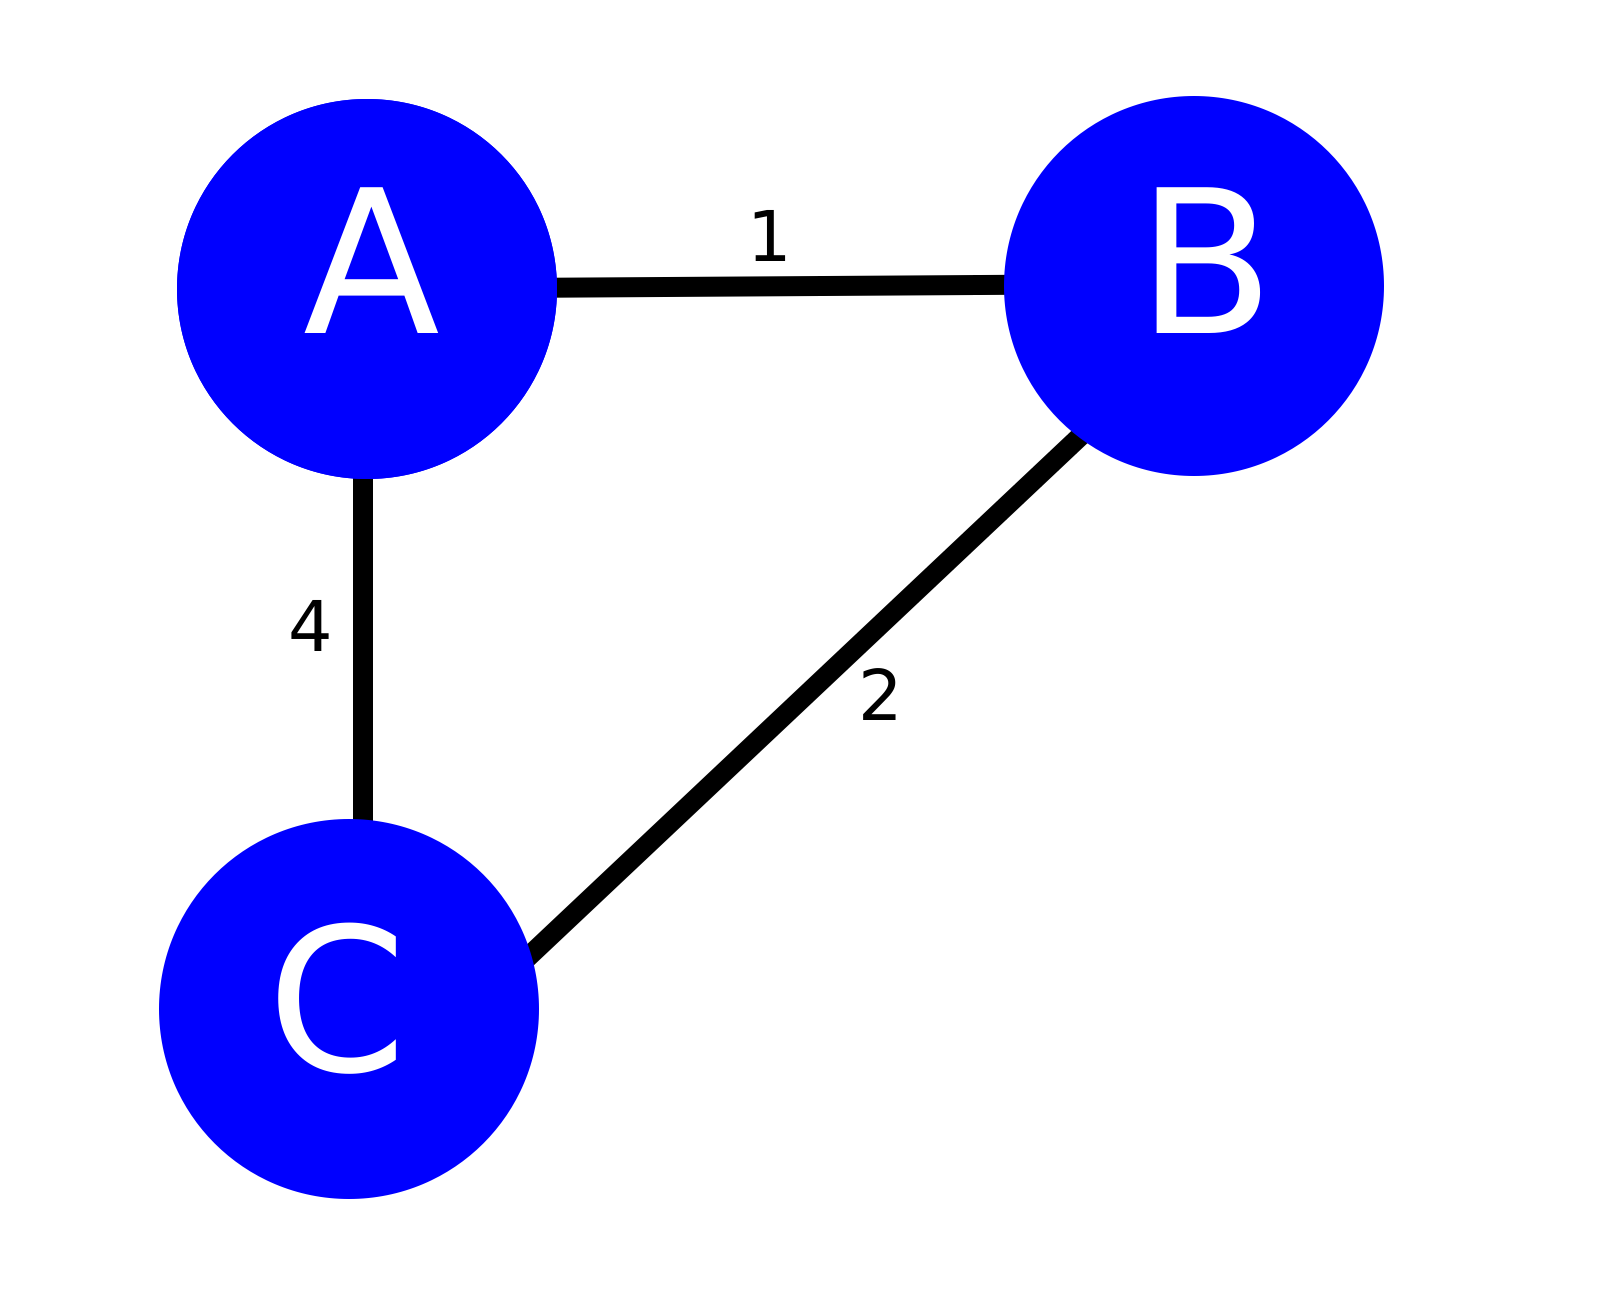
\includegraphics[width=0.5\textwidth]{img/img1.png}
    \caption{Rete iniziale con nodi A, B, C.}
    \label{fig:initial_network}
\end{figure}

Successivamente, esegue la simulazione del Distance Vector Routing, che consiste nell'inizializzare le tabelle di routing e propagare gli aggiornamenti fino alla convergenza La tabella di routing iniziale è mostrata nella Figura \ref{fig:initial_routing_table_1}. La tabella finale è mostrata nella Figura \ref{fig:final_routing_table_1}

\begin{figure}[H]
    \centering
    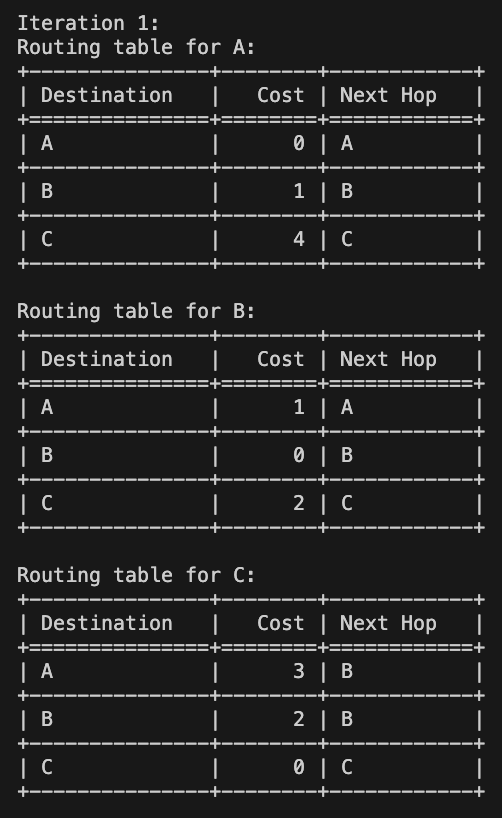
\includegraphics[width=0.4\textwidth]{img/rete1inizio.png}
    \caption{Tabella di routing iniziale per i nodi A, B, C.}
    \label{fig:initial_routing_table_1}
\end{figure}

\begin{figure}[H]
    \centering
    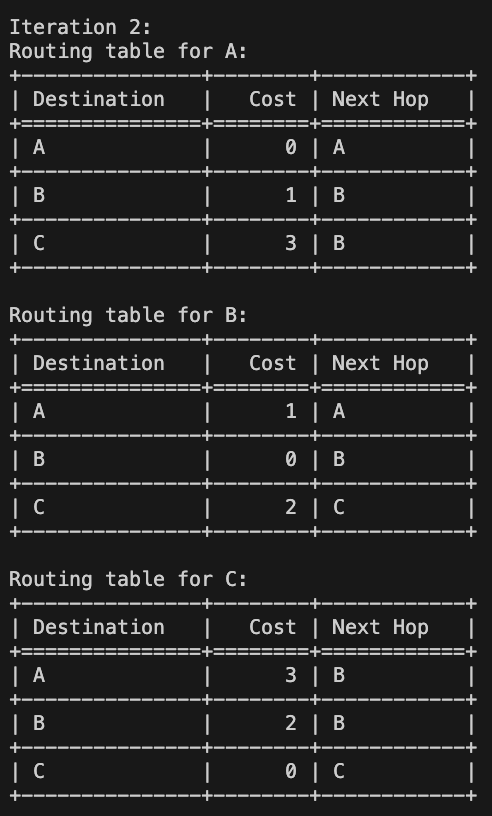
\includegraphics[width=0.4\textwidth]{img/rete1fine.png}
    \caption{Tabella di routing finale per i nodi A, B, C.}
    \label{fig:final_routing_table_1}
\end{figure}

\section{Modifica della Rete}
Dopo la prima simulazione, lo script modifica dinamicamente la rete aggiungendo un nuovo nodo (\texttt{D}), collegandolo ai nodi esistenti con costi specificati, e rimuovendo il collegamento tra B e C. La rete modificata è mostrata nella Figura \ref{fig:modified_network_1}.

\begin{figure}[H]
    \centering
    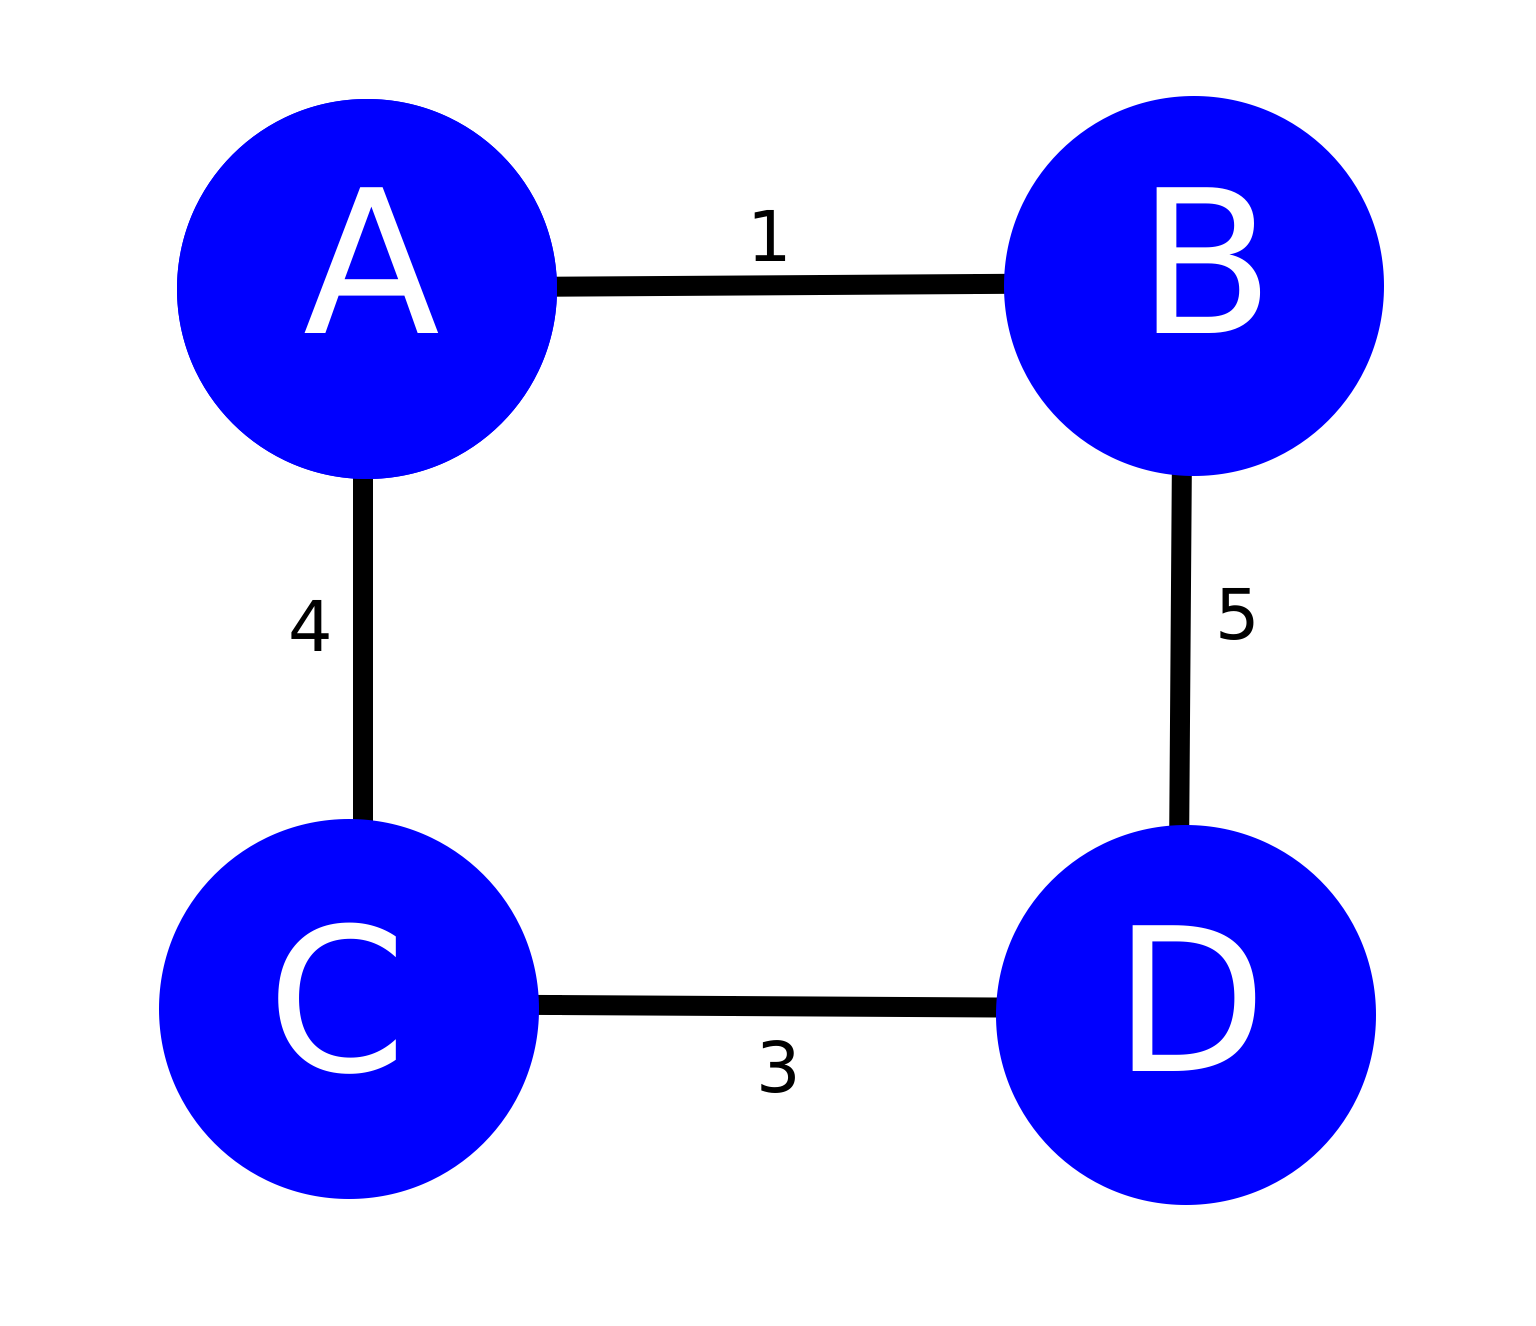
\includegraphics[width=0.5\textwidth]{img/img2.png}
    \caption{Rete modificata con l'aggiunta del nodo D e la rimozione del collegamento tra B e C.}
    \label{fig:modified_network_1}
\end{figure}

La simulazione viene quindi rieseguita per riflettere i cambiamenti. La tabella di routing iniziale è mostrata nella Figura \ref{fig:initial_routing_table_2}. La tabella finale è mostrata nella Figura \ref{fig:final_routing_table_2}

\begin{figure}[H]
    \centering
    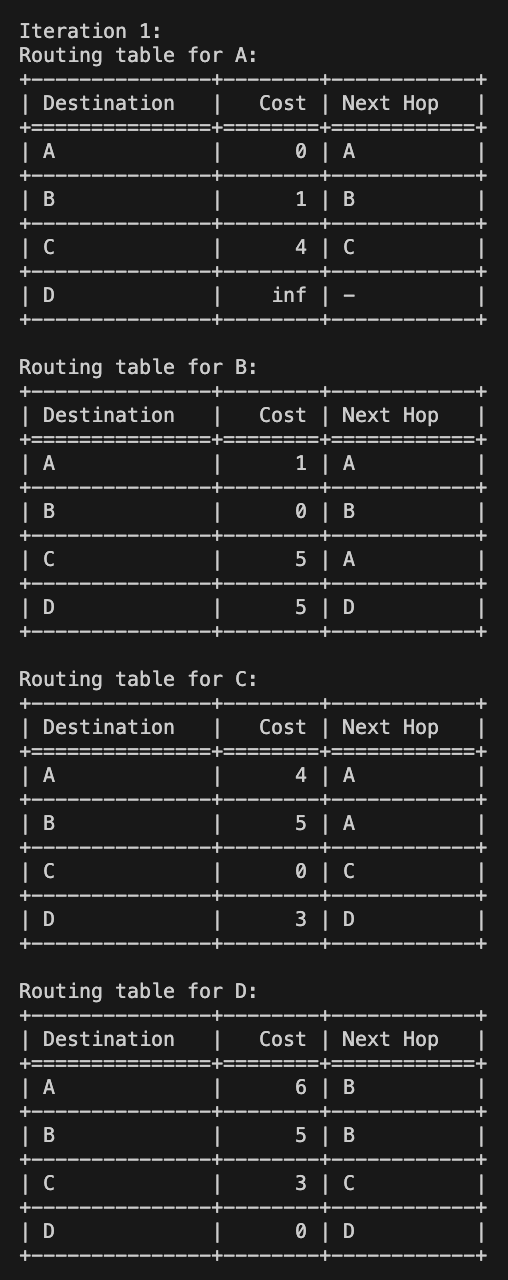
\includegraphics[width=0.6\textwidth]{img/rete2inizio.png}
    \caption{Tabella di routing iniziale per i nodi A, B, C, D.}
    \label{fig:initial_routing_table_2}
\end{figure}

\begin{figure}[H]
    \centering
    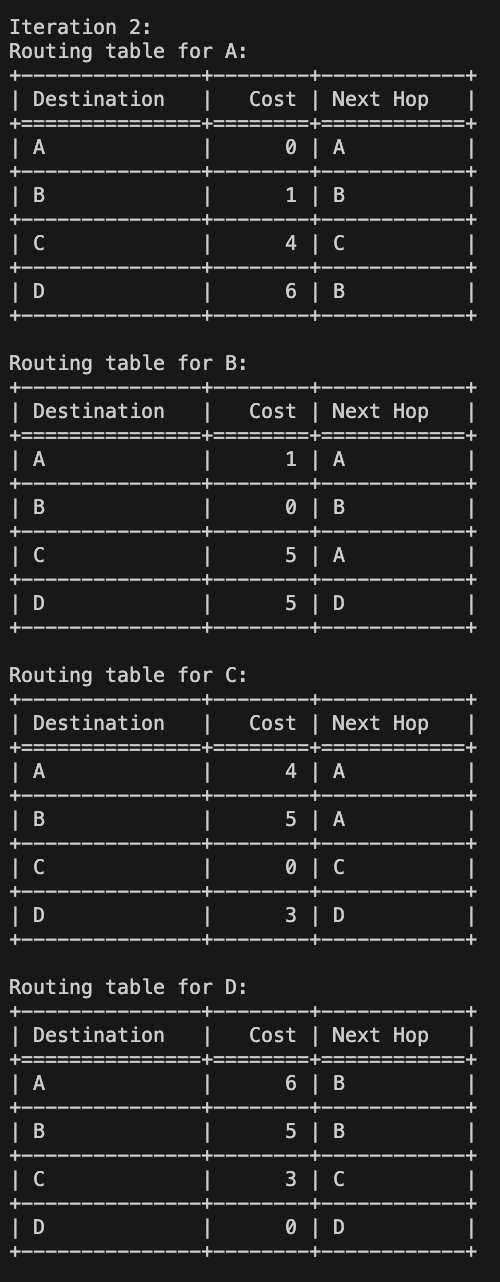
\includegraphics[width=0.6\textwidth]{img/rete2fine.png}
    \caption{Tabella di routing finale per i nodi A, B, C, D.}
    \label{fig:final_routing_table_2}
\end{figure}

\section{Ulteriore Modifica della Rete}
Infine, lo script modifica il costo di un collegamento esistente e riesegue la simulazione per aggiornare le tabelle di routing. La rete con il costo modificato è mostrata nella Figura \ref{fig:modified_network_2}.

\begin{figure}[H]
    \centering
    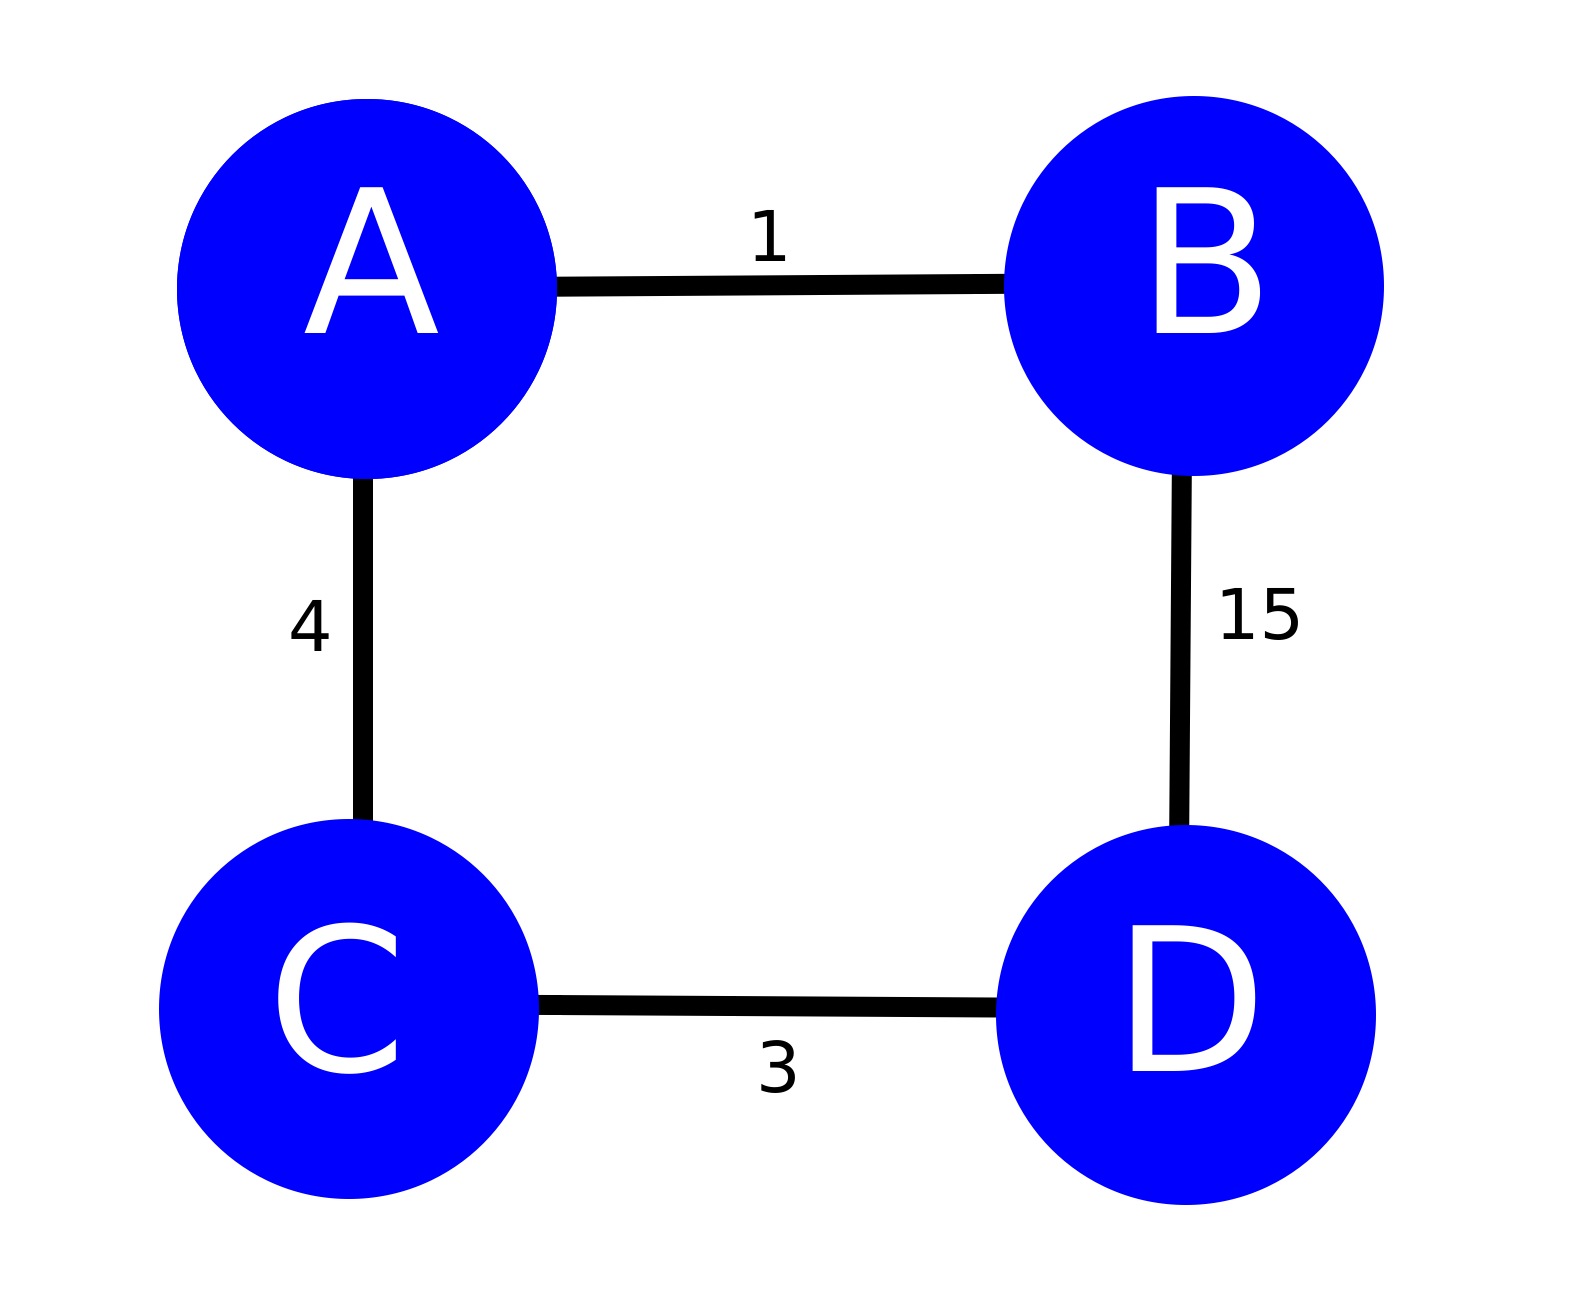
\includegraphics[width=0.5\textwidth]{img/Img3.png}
    \caption{Rete con il costo del collegamento tra B e D modificato.}
    \label{fig:modified_network_2}
\end{figure}

La simulazione viene quindi rieseguita per riflettere i cambiamenti causati dalla modifica del costo dell'arco. La tabella di routing iniziale è mostrata nella Figura \ref{fig:initial_routing_table_3}. La tabella finale è mostrata nella Figura \ref{fig:final_routing_table_3}

\begin{figure}[H]
    \centering
    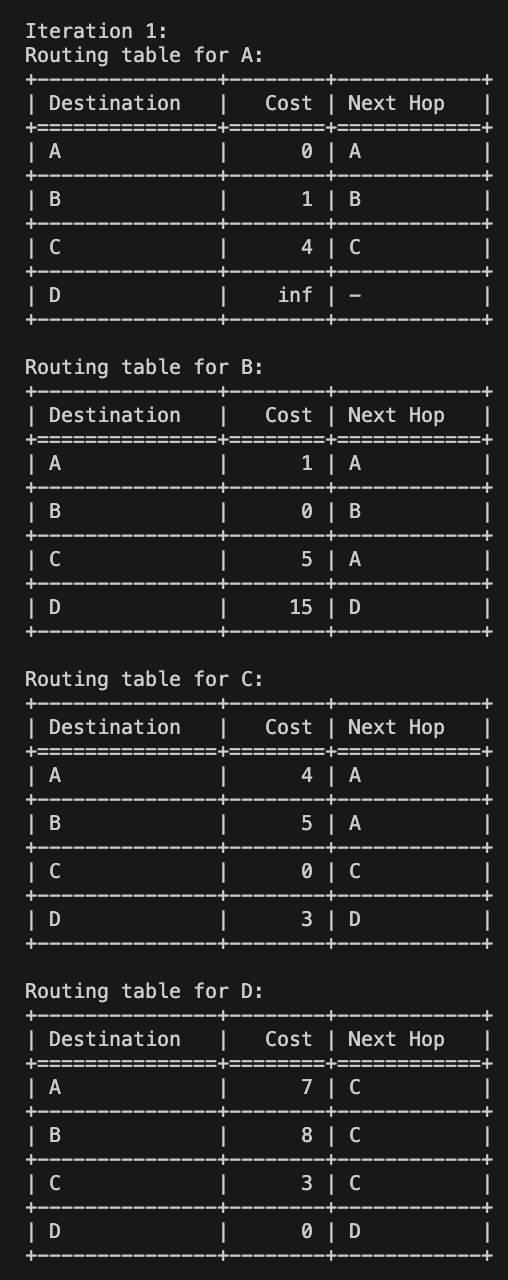
\includegraphics[width=0.6\textwidth]{img/rete3inizio.png}
    \caption{Tabella di routing iniziale per i nodi A, B, C, D dopo il cambio di costo.}
    \label{fig:initial_routing_table_3}
\end{figure}

\begin{figure}[H]
    \centering
    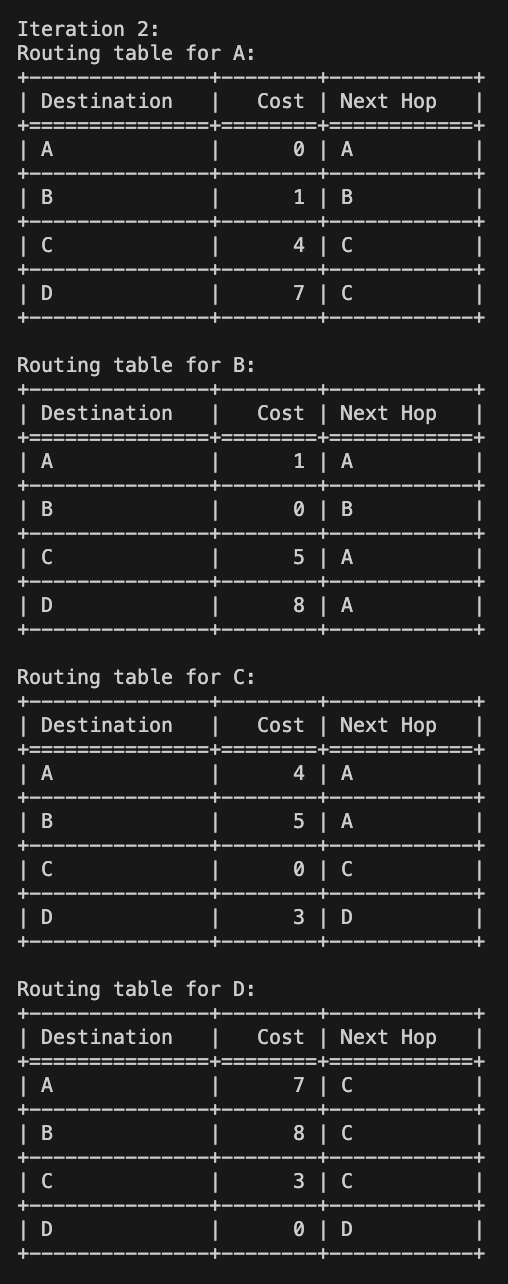
\includegraphics[width=0.6\textwidth]{img/rete3fine.png}
    \caption{Tabella di routing finale per i nodi A, B, C, D dopo il cambio di costo.}
    \label{fig:final_routing_table_3}
\end{figure}

\chapter{Conclusione}
Questo script fornisce una semplice ma efficace simulazione del protocollo di routing Distance Vector, permettendo di osservare come le tabelle di routing vengono aggiornate in risposta ai cambiamenti nella topologia della rete. Le funzioni modulari e ben definite rendono lo script facilmente estendibile per ulteriori esperimenti e simulazioni.

\end{document}